
\documentclass{report}

\usepackage[utf8]{inputenc}
\usepackage[italian]{babel}
\usepackage{import}
\usepackage{todonotes}
\usepackage{color}
\usepackage{rotating}
\usepackage[hidelinks]{hyperref}
\usepackage{url}
\usepackage{pdfpages}
\usepackage{siunitx}
\usepackage{pdflscape}
\usepackage{subfig}
\usepackage[euler]{textgreek}
\usepackage{mhchem}

\usepackage{enumerate} 
\usepackage{amsmath}
\usepackage{amsfonts}

\usepackage[signatures,swapnames,sans]{frontespizio}

\usepackage{geometry}
\geometry{portrait, margin=3cm}
\usepackage{siunitx}
\usepackage{booktabs}

\renewcommand*\figurename{Figura}

\newcommand{\sub}[1]{\textsubscript{#1}}
\newcommand{\super}[1]{\textsuperscript{#1}}
\newcommand{\parallelsum}{\mathbin{\!/\mkern-5mu/\!}}

\newcommand{\Fig}[0]{Fig.}

\usepackage{titlesec}

\titleformat{\chapter}{\normalfont\huge}{}{20pt}{\huge\bfseries}

\linespread{1.3}

\begin{document}
	\begin{frontespizio}
		\Margini{3cm}{3cm}{3cm}{3cm}
		\Universita{Bergamo}
		\Logo[43.332mm]{unibg-mark}
		\Divisione{Scuola di Ingegneria}
		\Corso[Laurea Magistrale]{Ingegneria Informatica}
		\Titolo{Laboratorio di Elettronica}
		\Sottotitolo{Relazione esperienza di laboratorio 1}
		\Punteggiatura{}
		\NRelatore{Prof.}{Prof.}
		\Relatore{Luigi Gaioni}
		\Candidato[1058231]{Giulia Allievi}
		\Candidato[1059640]{Martina Fanton}
		\Annoaccademico{2022--2023}
		\begin{Preambolo*}
			\usepackage[italian]{babel}
			\usepackage[T1]{fontenc}
			\usepackage[utf8]{inputenc}
			\usepackage{microtype}
			\usepackage{lmodern}
			\graphicspath{{img/}}
			
			\renewcommand{\frontinstitutionfont}{\fontsize{14}{17}\bfseries\scshape}
			\renewcommand{\fronttitlefont}{\fontsize{17}{21}\bfseries\scshape}
			\renewcommand{\frontfootfont}{\fontsize{12}{14}\bfseries\scshape}
		\end{Preambolo*}
	\end{frontespizio}

%----------------------------------------------------------------------------------------
%	PAGINA BIANCA
%----------------------------------------------------------------------------------------
\newpage
\null
\thispagestyle{empty}
\newpage

%----------------------------------------------------------------------------------------
%	INTRO
%----------------------------------------------------------------------------------------
\chapter{Filtro passa-basso attivo}
\section{Introduzione}
% circuito da realizzare
% uA741
% spiegazione veloce pin
Il primo circuito che abbiamo realizzato è un filtro passa-basso attivo. Per costruire questo circuito abbiamo bisogno di un amplificatore operazionale, nel nostro caso abbiamo scelto il \textmu A741, che è un amplificatore operazionale \textit{general purpose}. Per funzionare correttamente, dobbiamo fornirgli sia un'alimentazione positiva che un'alimentazione negativa perché è un componente attivo ad alimentazione duale. Nell'immagine sottostante, la figura \ref{figura:741}, si possono vedere i numeri e la funzione di ogni terminale di questo componente. Per capire quali sono i terminali, sul package troviamo un pallino in corrispondenza del pin numero 1.  \par
\begin{figure}[h]
\centering
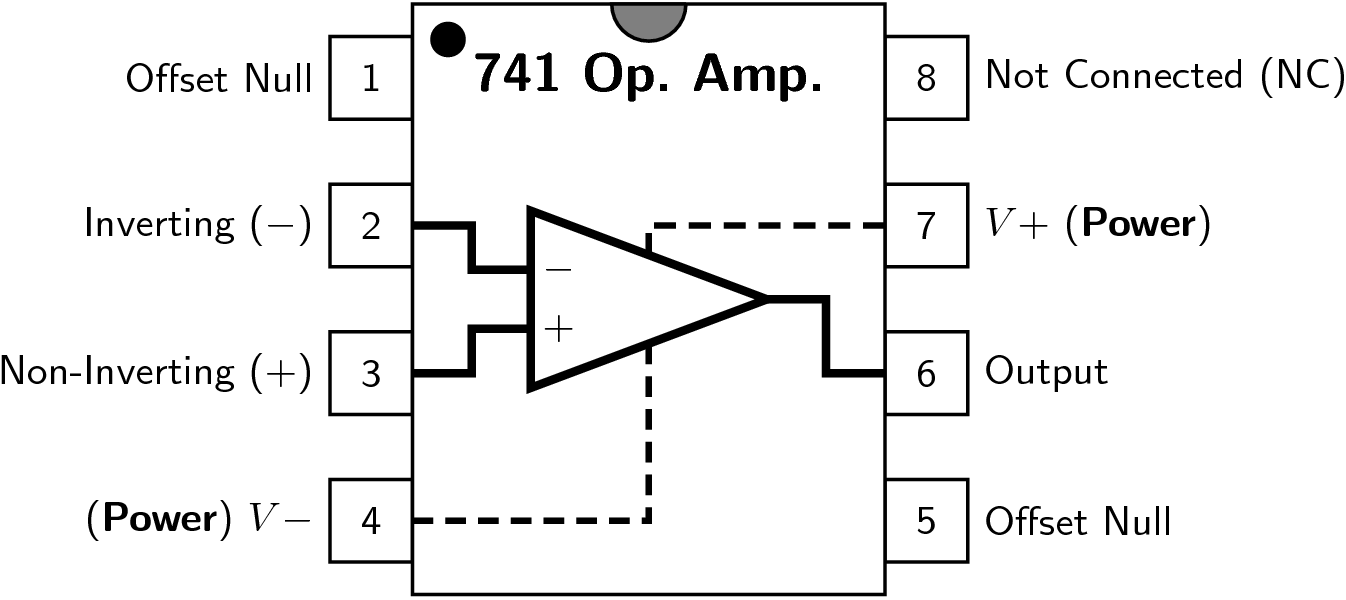
\includegraphics[height=6cm]{immagini/741pinout}
\caption{Package e funzione dei pin del \textmu A741.}
\label{figura:741}
\end{figure}
\section{Schema del circuito e analisi teorica}
%% Analisi (da EMI)
\noindent Per analizzare questo circuito facciamo riferimento alla figura \ref{figura:cto_analisi}.
\begin{figure}[h]
\centering
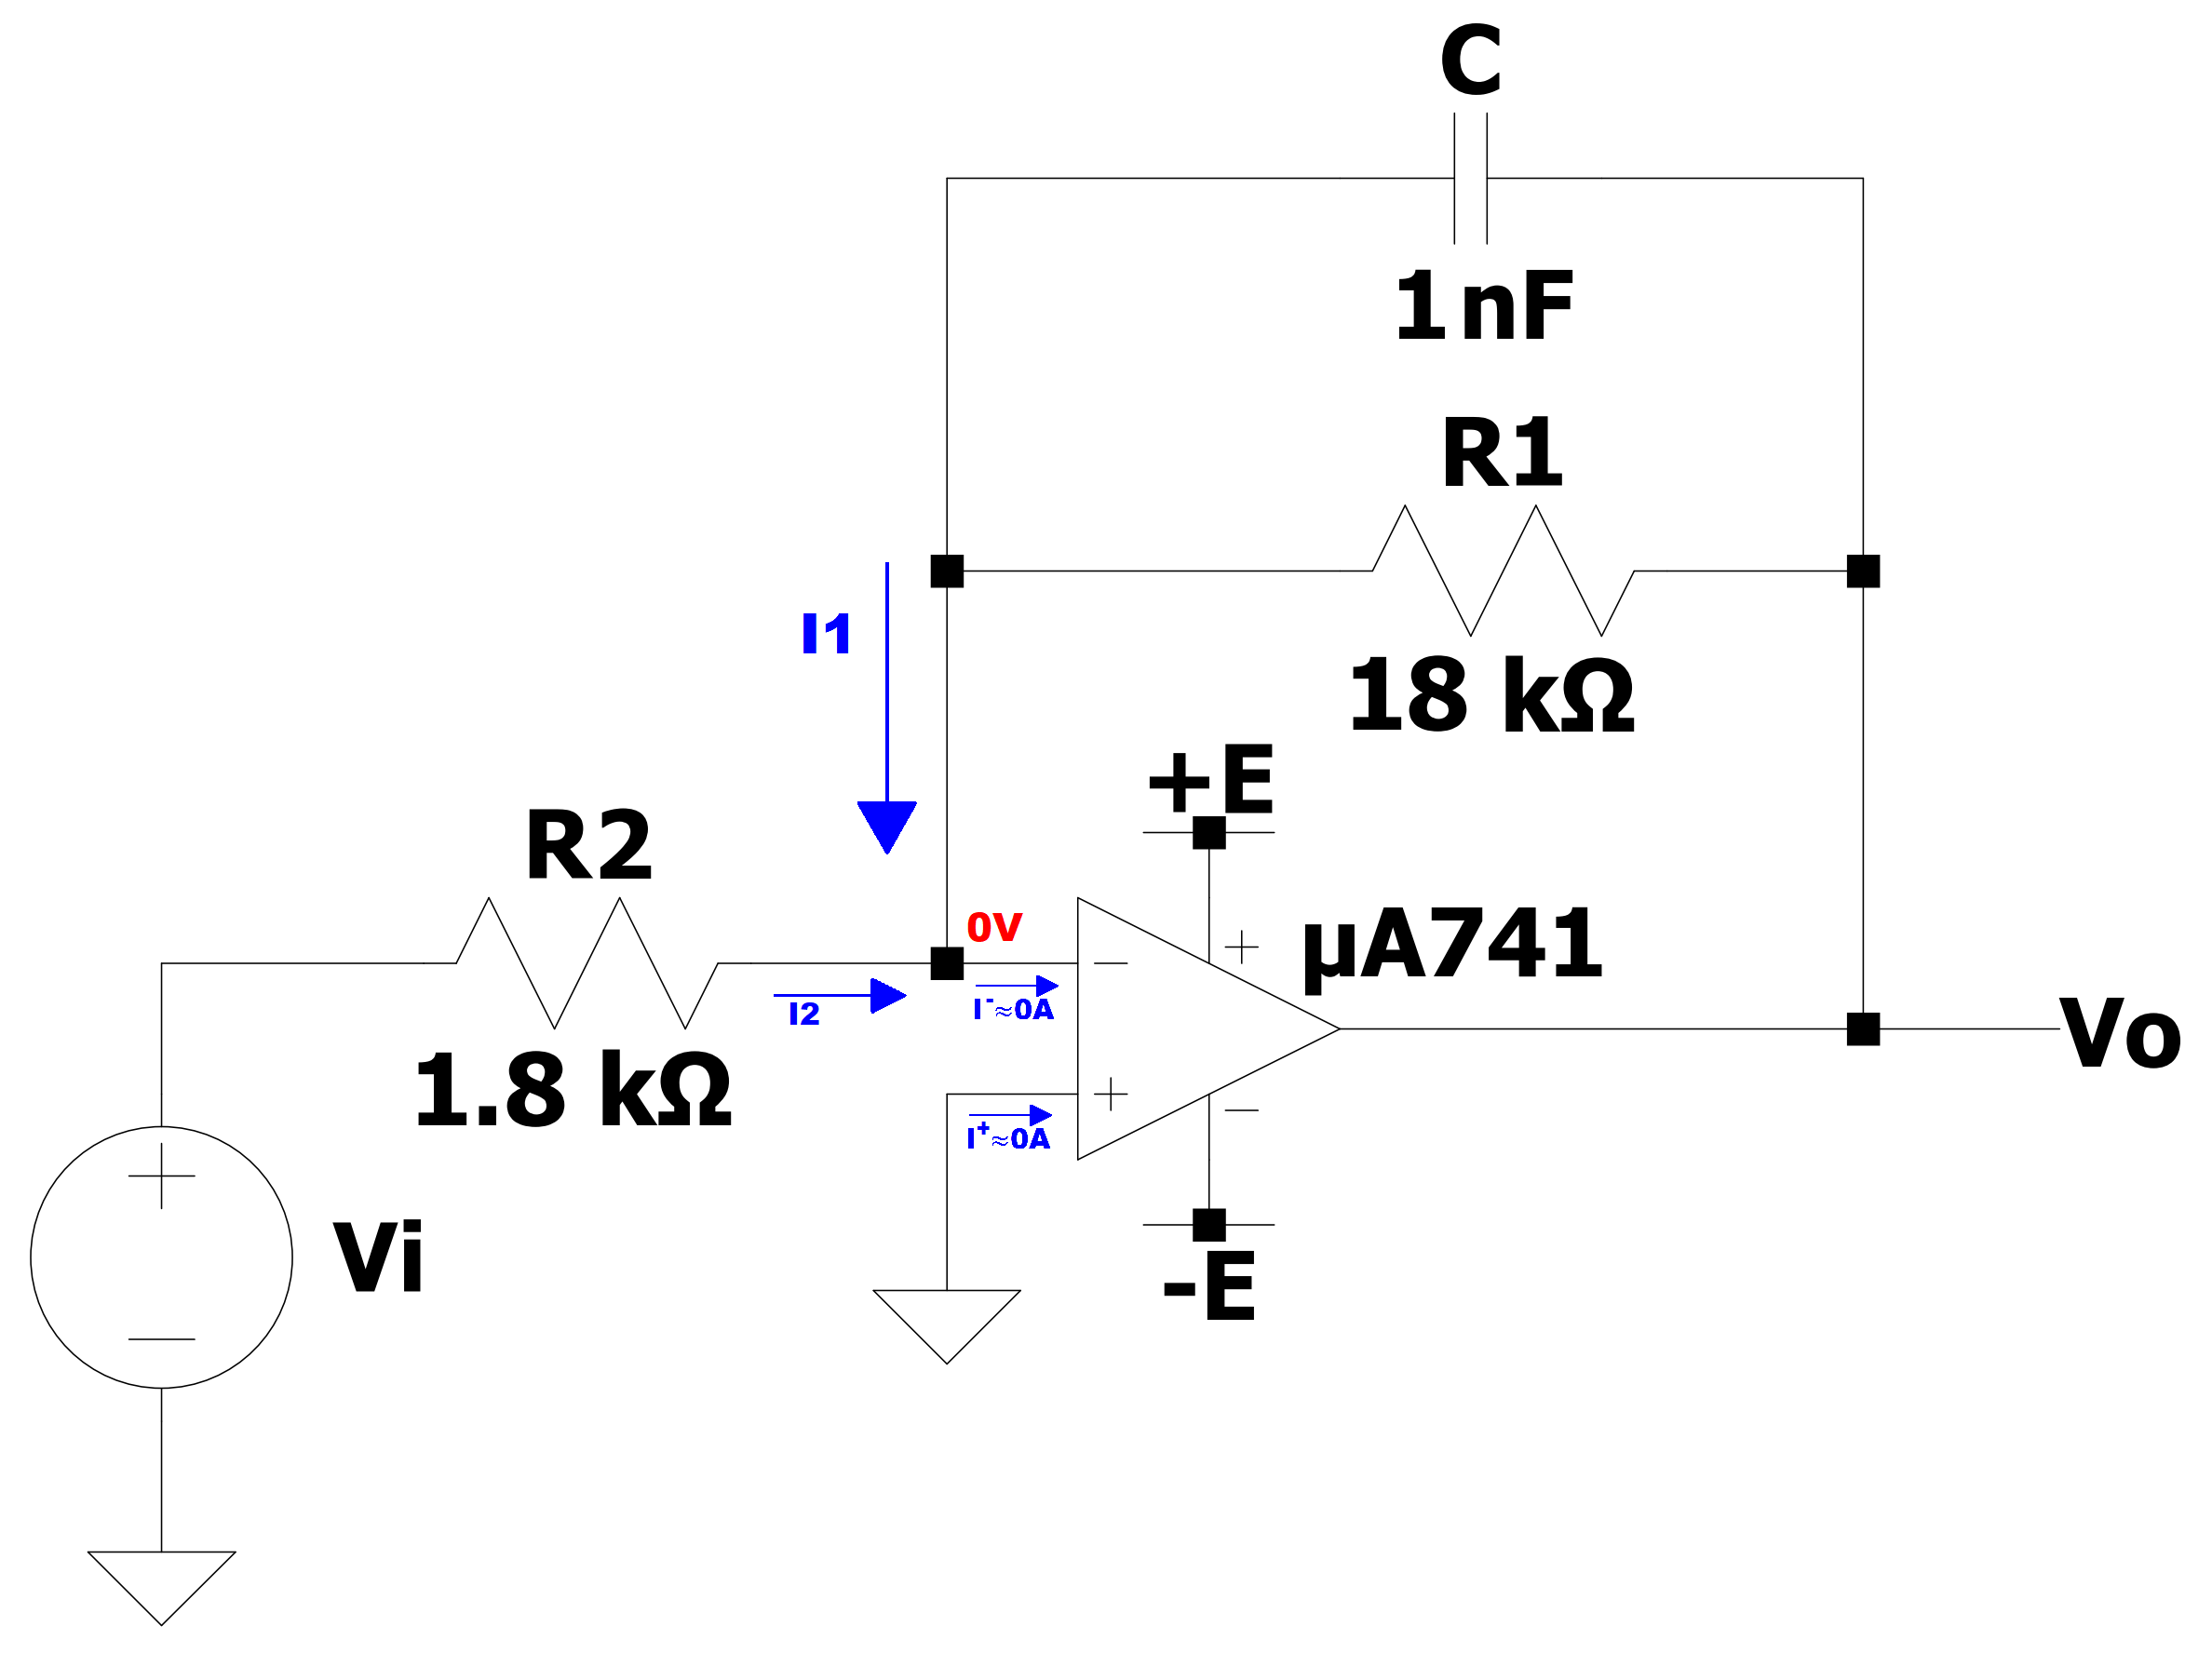
\includegraphics[height=8cm]{immagini/cto_filtro_analisi}
\caption{Schema per analizzare il filtro.}
\label{figura:cto_analisi}
\end{figure}
La resistenza $R_1$ e il condensatore $C_1$ sono in parallelo, pertanto si può calcolare l'impedenza equivalente:
\\[4pt]\indent$\displaystyle{Z_{eq}=C_1\parallelsum R_1=\frac{\frac{1}{s\cdot C_1} \cdot R_1}{\frac{1}{s\cdot C_1} + R_1}=\frac{\frac{R_1}{s\cdot C_1}}{\frac{1+s\cdot R_1C_1}{s\cdot C_1}}=\frac{R_1}{1+s\cdot R_1C_1}}$
\newpage \noindent Per ricavare la funzione di trasferimento del circuito è sufficiente fare un bilancio di correnti all'ingresso invertente: 
\\[2pt]\indent $I_2=I_1+I^-$ \indent (con $I_1$ si intende la corrente che scorre nell'impedenza equivalente $Z_{eq}$)
\\[2pt]La corrente in ingresso all'OPAMP è molto piccola, idealmente $I^+=I^-\rightarrow 0A$. Perciò l'equazione precedente diventa:
\\\indent $\displaystyle{I_2=I_1}$
\\Utilizzando la legge di Ohm generalizzata, le correnti si possono esprimere come:
\\[2pt]\indent $\displaystyle{\frac{V_i(s)-V^-(s)}{R_2}=(V^-(s)-V_o(s))\cdot\frac{1+s\cdot R_1C_1}{R_1}}$
\\[2pt]Se un circuito è retroazionato negativamente, $V^+=V^-$ per il principio del cortocircuito virtuale. Dato che $V^+$ è a massa, la sua tensione è di 0V, di conseguenza anche $V^-$ si troverà a questa tensione. L'equzione precedente diventa:
\\[2pt]\indent $\displaystyle{\frac{V_i(s)}{R_2}=-V_o(s)\cdot\frac{1+s\cdot R_1C_1}{R_1}}$
\\[2pt]Tramite quest'equazione è facile ricavare la funzione di trasferimento del circuito, che risulta:
\\[2pt]\indent $\displaystyle{\frac{V_o(s)}{V_i(s)}=-\frac{R_1}{R_2}\cdot\frac{1}{1+s\cdot R_1C_1}}$
\\[2pt]La funzione di trasferimento ottenuta è quella di un filtro passa-basso, perché al denominatore troviamo il termine $1+s\cdot R_1C_1$. Vediamo che c'è però anche un fattore di guadagno pari al rapporto fra $R_1$ e $R_2$. Compare anche un segno meno, pertanto l'ingresso e l'uscita saranno sfasate di $\displaystyle\pm$180°.
\\Se passiamo al regime sinusoidale, sostituiamo $s$ con $j\omega$. La funzione di trasferimento diventa:
\\[2pt]\indent $\displaystyle{\frac{V_o(\omega)}{V_i(\omega)}=-\frac{R_1}{R_2}\cdot\frac{1}{1+j\omega\cdot R_1C_1}}$
\\[2pt]La frequenza di taglio del filtro è pari a $\displaystyle{f_T=\frac{1}{2\pi\cdot R_1C_1}}$. A questa frequenza il guadagno si riduce di 3 dB e lo sfasamento è di $\mp$45°.
\\[2pt]Se lavoriamo a frequenze minori della frequenza di taglio del filtro, il termine passa-basso è trascurabile, perciò la funzione di trasferimento si semplifica:
\\[2pt]\indent$\displaystyle{\frac{V_o}{V_i}=-\frac{R_1}{R_2}}$
\\[2pt]Vediamo che il guadagno dipende dal rapporto fra le due resistenze: se $R_1<R_2$ il circuito attenua il segnale in ingresso, quindi otteniamo un attenuatore (invertente); se $R_1>R_2$ il segnale viene amplificato, perciò il circuito si comporta come un amplificatore (invertente); infine, se $R_1=R_2$ il circuito ha guadagno unitario, di conseguenza si comporta come un buffer (invertente). 
\section{Dimensionamento, misure e osservazioni}
Per alimentare l'amplificatore operazionale abbiamo utilizzato un'alimentazione duale, con tensione positiva di \SI{10}{\volt} e alimentazione negativa di \SI{-10}{\volt}. L'obiettivo è realizzare un filtro con frequenza di taglio dell'ordine di \SI{10}{k\hertz} e guadagno 10. \par
\noindent Per il dimensionamento scegliamo $R_1=\SI{18}{k\ohm}$ e calcoliamo $R_2$ dalla formula del guadagno:
\\[2pt]\indent$\displaystyle{G=\frac{R_1}{R_2}\rightarrow R_2=\frac{R_1}{G} = \frac{\SI{18}{k\ohm}}{10}=\SI{1.8}{k\ohm}}$ 
\\[2pt]Dalla frequenza di taglio desiderata calcoliamo il valore che deve avere la capacità $C_1$:
\\[2pt]\indent$\displaystyle{f_T=\frac{1}{2\pi\cdot R_1C_1}\rightarrow C_1=\frac{1}{2\pi\cdot R_1\cdot f_T}=\frac{1}{2\pi\cdot \SI{18}{k\ohm}\cdot \SI{10}{k\hertz}}\simeq\SI{0.88}{n\farad}}$
\\[4pt]Scegliamo di approssimare $C_1$ a \SI{1}{n\farad}, perciò la frequenza di taglio del nostro filtro sarà:
\\[2pt]\indent$\displaystyle{f_T=\frac{1}{2\pi\cdot R_1C_1}=\frac{1}{2\pi\cdot \SI{18}{k\ohm}\cdot \SI{1}{n\farad}}\simeq\SI{8.84}{k\hertz}}$ % MOD (aggiunta una cifra significativa a f_T)
\\[4pt]In figura \ref{figura:cto_filtro} è riportato lo schema del circuito con i valori dei componenti scelti. 
\begin{figure}[h!]
\centering
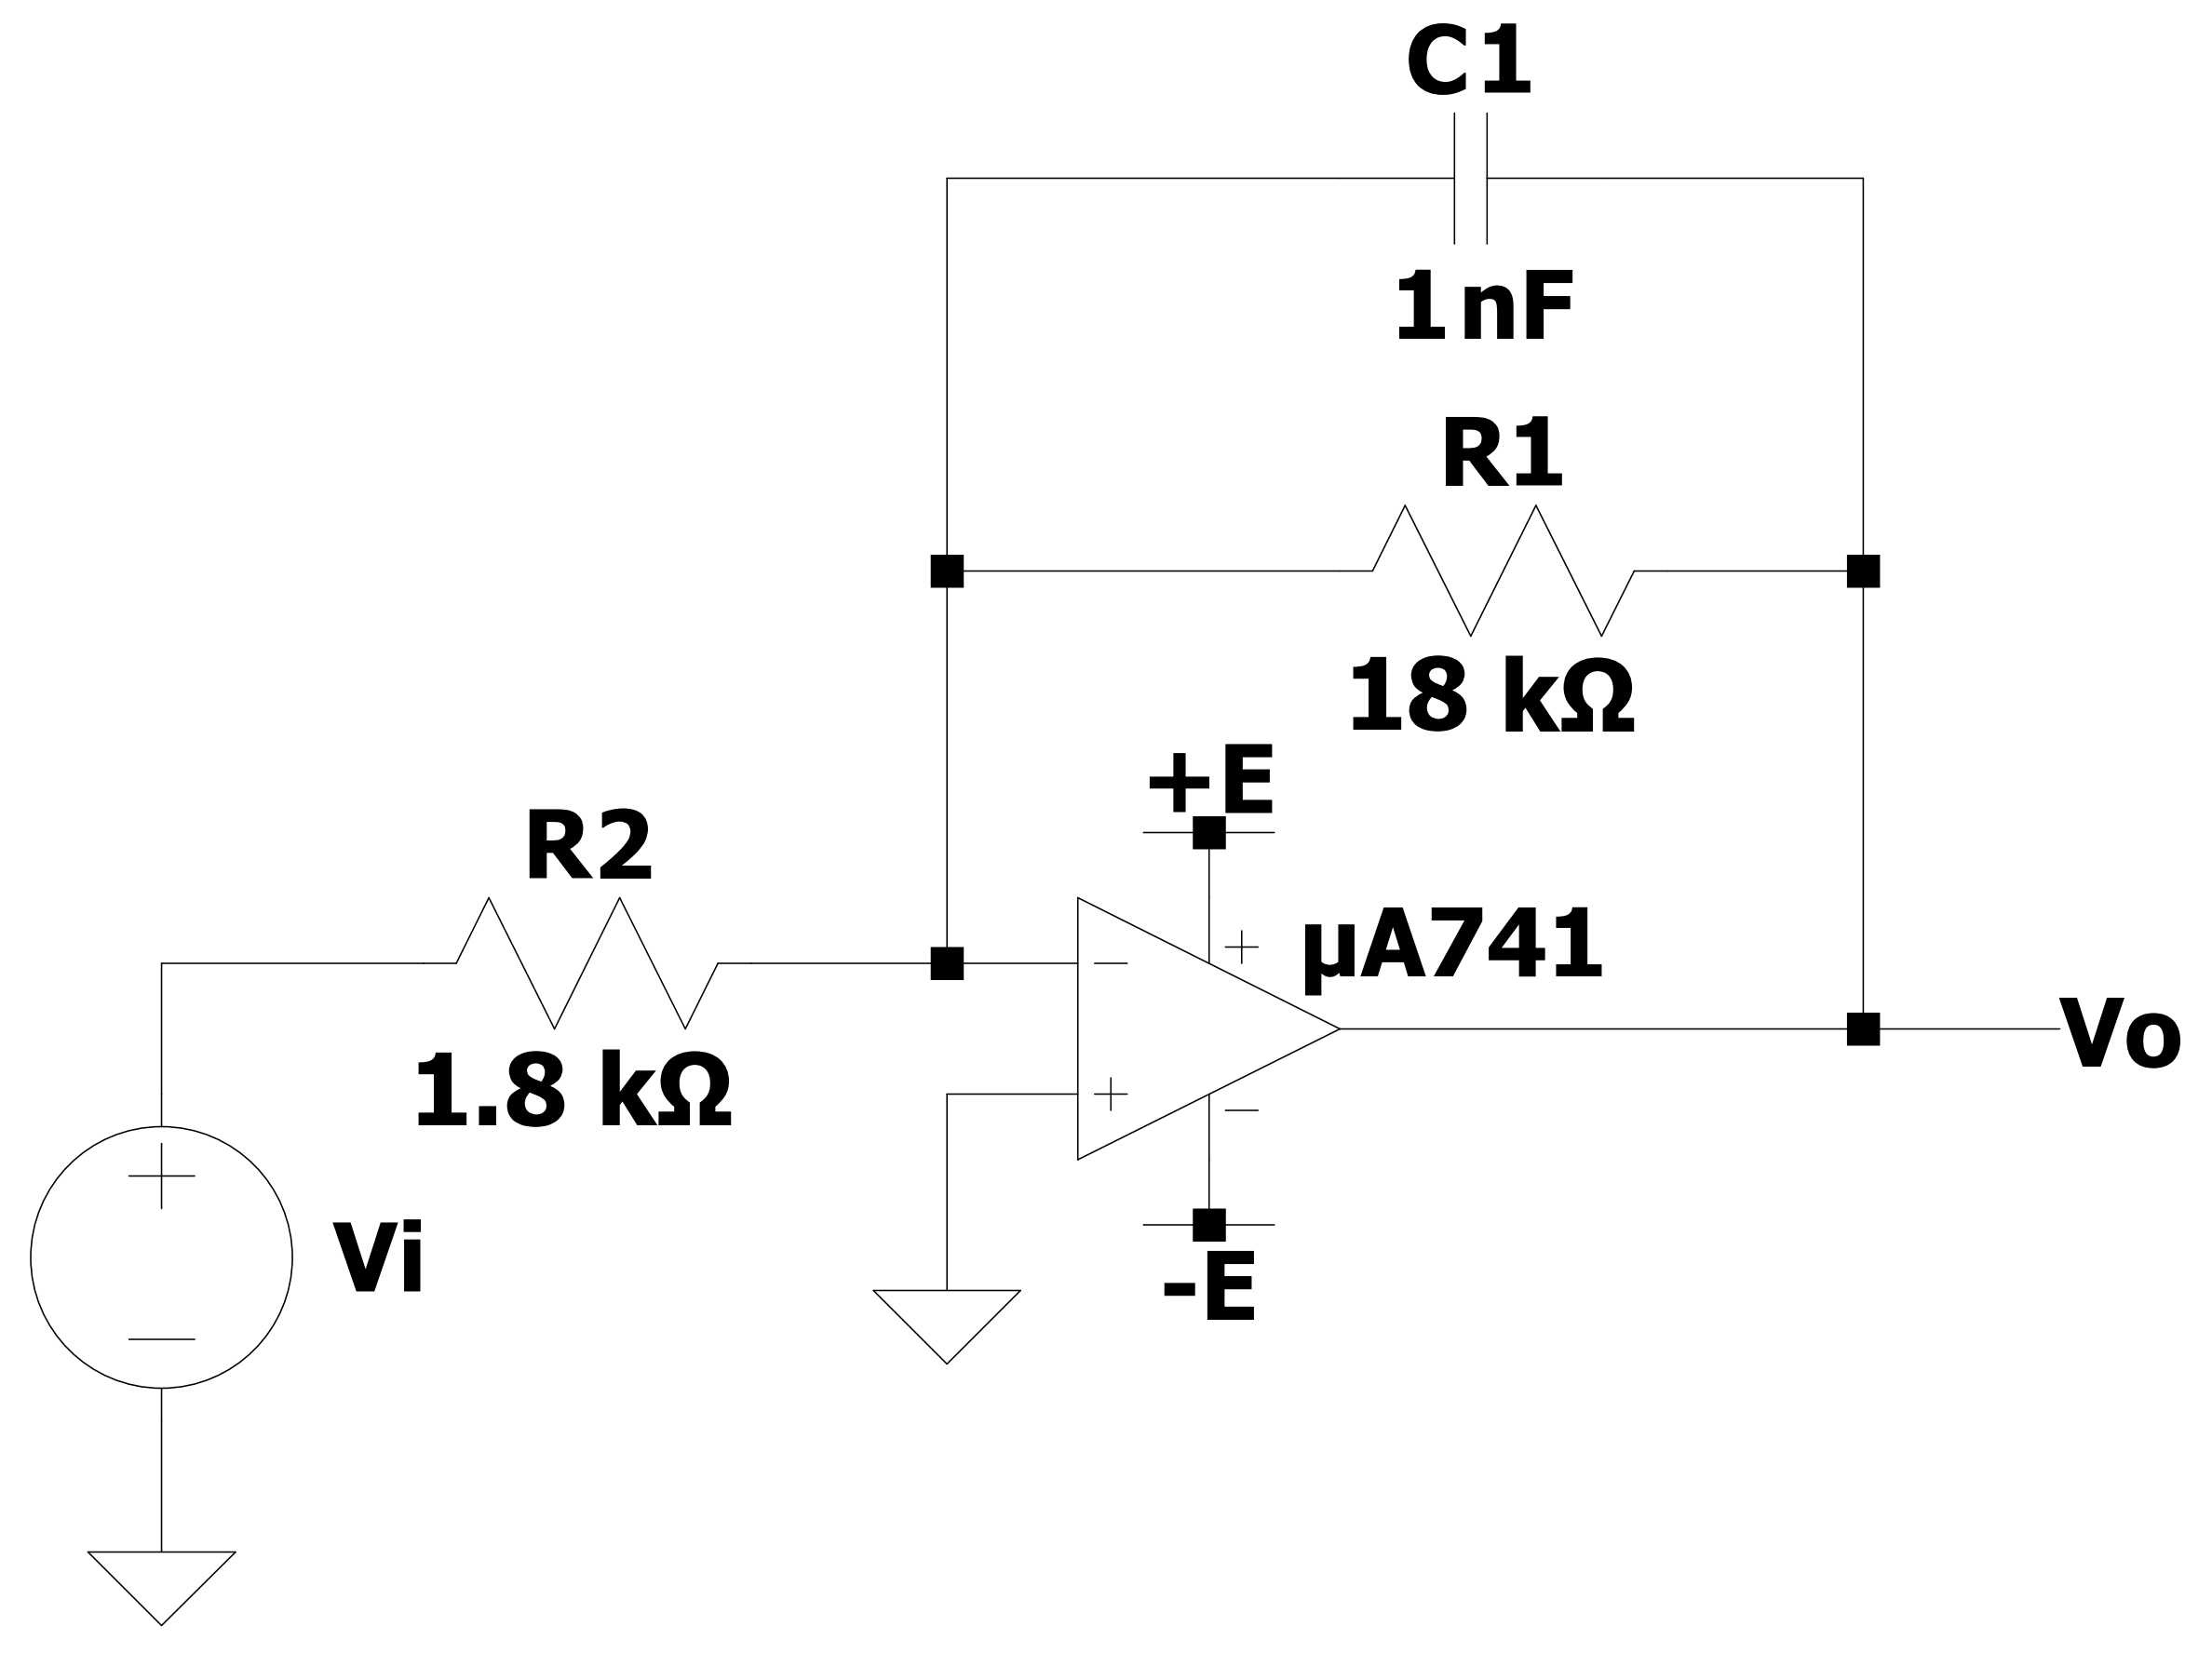
\includegraphics[height=8cm]{immagini/cto_filtro}
\caption{Schema del filtro passa-basso attivo con i valori scelti.}
\label{figura:cto_filtro}
\end{figure}
\\Con il multimetro andiamo a misurare il valore delle resistenze che monteremo sulla breadboard. Le misure sono riportate in tabella \ref{table:mis_res}.
\begin{table}[h]
	\centering
	\begin{tabular}{|c|c|c|}
	\cline{2-3} 
	\multicolumn{1}{c|}{} & \textbf{Valore nominale} & \textbf{Valore misurato}\\ 
		%\hline
		%{} & \textbf{Valore nominale} & \textbf{Valore misurato} \\ 
		\hline
		$\mathbf{R_1}$ & \SI{18}{k\ohm} & \SI{17.977}{k\ohm} \\ 
		\hline
		$\mathbf{R_2}$& \SI{1.8}{k\ohm} & \SI{1.815}{k\ohm} \\ 
		\hline
	\end{tabular}
\caption{Misure delle resistenze utilizzate per il circuito.}
\label{table:mis_res}
\end{table}
\\Per realizzare il filtro posizioniamo il \textmu A741 sulla breadboard e colleghiamo i terminali in questo modo:
\begin{itemize}
\item i terminali 1 e 5 servono per compensare l'offset, li lasciamo floating;
\item il terminale 2 è l'ingresso invertente. A questo terminale colleghiamo un terminale della resistenza $R_1$ e un terminale della capacità $C_1$, inoltre applichiamo il segnale tramite la resistenza $R_2$;
\item il terminale 3, ovvero l'ingresso non-invertente, lo connettiamo a massa;
\item i terminali 4 e 7 sono collegati rispettivamente all'alimentazione  negativa e all'alimentazione positiva;
\item il terminale 6 serve per prelevare l'output. Questo terminale è collegato al terminale di $R_1$ e al terminale di $C_1$ non connessi con il pin 2;
\item il terminale numero 8 è \textit{Not Connected}, perciò non viene collegato a nulla.
\end{itemize}
In figura \ref{figura:foto_circ} è mostrata una fotografia del circuito realizzato in cui si possono vedere le connessioni descritte in precedenza.
\begin{figure}[h!]
\centering
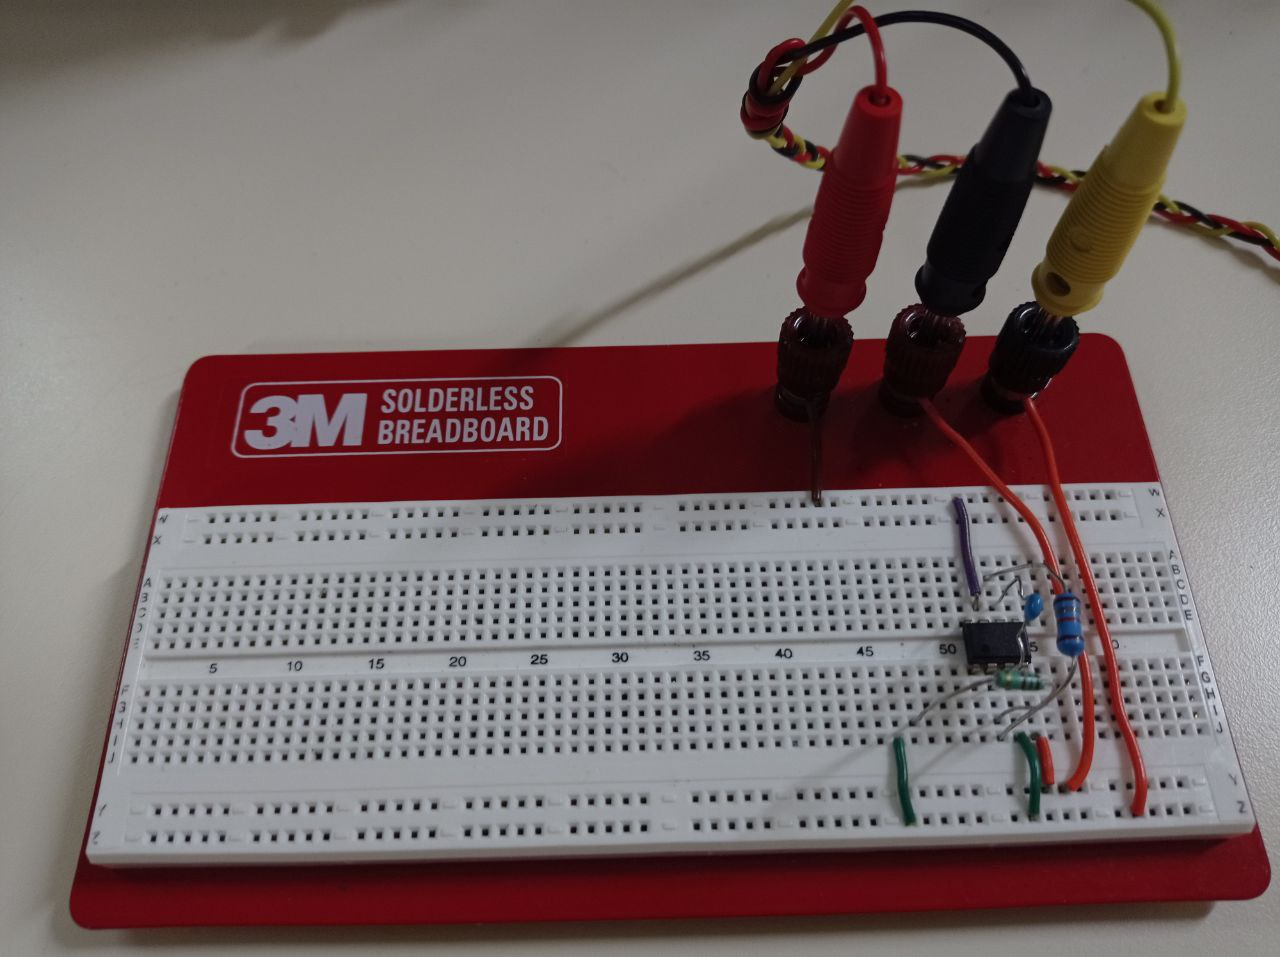
\includegraphics[height=7.6cm]{immagini/circuito}
\caption{Fotografia del filtro passa-basso attivo realizzato in laboratorio.}
\label{figura:foto_circ}
\end{figure}
\\Alimentiamo il circuito e applichiamo un segnale collegando con un cavo BNC il generatore di forme d'onda al circuito. Per osservare la risposta del filtro utilizziamo l'oscilloscopio collegando le due sonde come mostrato in figura \ref{figura:connessioni}. I coccodrilli delle due sonde li colleghiamo a massa, la punta della prima sonda (CH1, traccia gialla) la colleghiamo al capo della resistenza $R_2$ connesso al generatore di forme d'onda, mentre la punta dell'altra sonda (CH2, traccia azzurra) la connettiamo al terminale di $R_1$ connesso al pin 6 del \textmu A741.
\begin{figure}[h!]
\centering
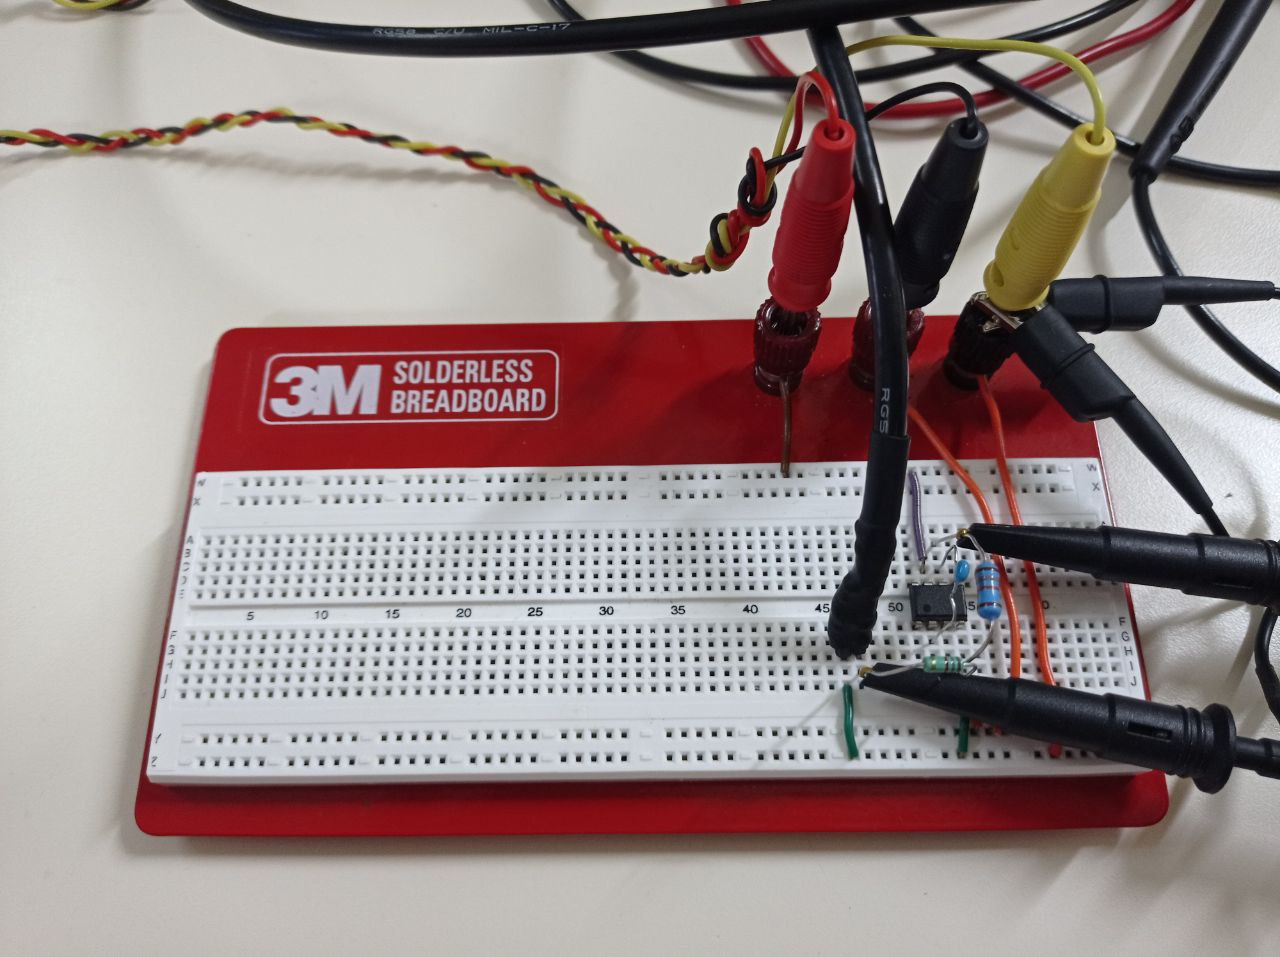
\includegraphics[height=7cm]{immagini/circuito_sonde}
\caption{Fotografia del filtro passa-basso attivo con le connessioni del segnale e dell'oscilloscopio.}
\label{figura:connessioni}
\end{figure}
\\Nella figura \ref{figura:TEK1} è mostrato il grafico prodotto dall'oscilloscopio in cui è rappresentata la risposta del circuito quando in ingresso applichiamo una sinusoide di frequenza \SI{100}{\hertz} e tensione picco-picco $V_{PP}=\SI{500}{m\volt}$.
\begin{figure}[h!]
	\centering
	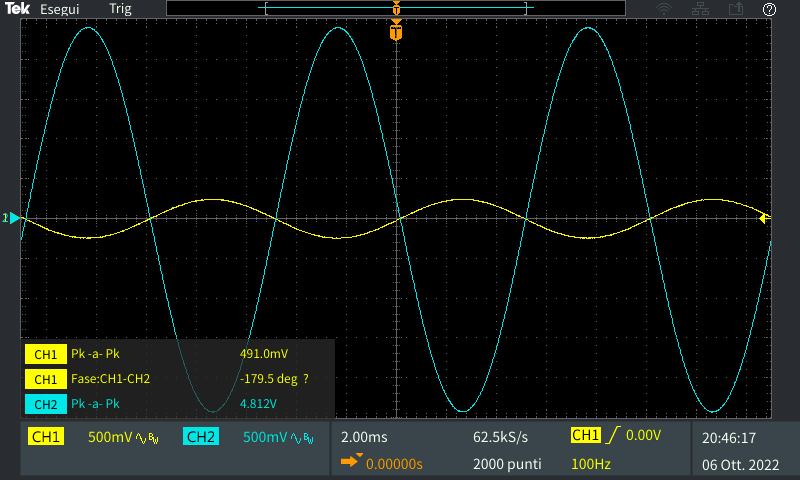
\includegraphics[height=6.5cm]{immagini/TEK00001}
	\caption{Grafico prodotto dall'oscilloscopio con una sinusoide di frequenza \SI{100}{\hertz}.}
	\label{figura:TEK1}
\end{figure}
\\Come si può notare dal grafico, la forma d'onda in ingresso presenta uno sfasamento rispetto alla forma d'onda in uscita pari a circa \SI{180}{\degree} e questo fatto è prevedibile poichè il circuito analizzato è in configurazione invertente. Infatti, quando il segnale in ingresso è positivo l'uscita è negativa, viceversa, quando l'ingresso è negativo l'uscita è positiva.\par % MOD
Se calcoliamo il guadagno (in modulo) del circuito otteniamo: $\displaystyle{G=\frac{V_{PP,out}}{V_{PP,in}}=\frac{\SI{4.812}{\volt}}{\SI{0.491}{\volt}}=9.80}$, quindi il guadagno del filtro è molto prossimo al valore che ci aspettiamo dalla teoria (è solo il 2\% in meno). Anche la frequenza di taglio ottenuta è confrontabile con la frequenza di taglio teorica, dato che superiore a questa di solo 0.1\%.\par % AGG
In seguito è stata svolta un'analisi sulla funzione sinusoidale scelta apportando delle variazioni alla frequenza e facendola variare in un intervallo compreso tra \SI{100}{\hertz} e \SI{10}{M\hertz}. I valori delle tensioni e della fase misurati con l'oscilloscopio ci serviranno per ricavare i diagrammi di Bode di modulo e fase del filtro, così da confrontarli con i diagrammi teorici per poter valutare le prestazioni del filtro. Le misure effettuate durante questa analisi sono state riportate nella tabella \ref{table:misure}. % MOD
\begin{table}[h!]
	\centering
	\begin{tabular}{|c|c|c|c|c|}
		\hline
		\textbf{Frequenza} &\boldmath$\displaystyle\mathrm{{V_{PP,in}}}$ \textbf{[V]} & \boldmath$\displaystyle\mathrm{{V_{PP,out}}}$\textbf{[V]} & \textbf{Guadagno} & \textbf{Sfasamento [°]}\\
		\hline
		100 Hz & 0.491 & 4.812 & 9.80 & -179.5\\
		\hline
		500 Hz & 0.488 & 4.799 & 9.83 & -176.8\\
		\hline
		1 kHz & 0.485 & 4.779 & 9.85 & -173.4\\
		\hline
		5 kHz & 0.481 & 4.188 & 8.71 & -149.7\\
		\hline
		8.8 kHz & 0.484 & 3.388 & 7.00 & -133.9\\
		\hline
		10 kHz & 0.485 & 3.163 & 6.52 & -129.7\\
		\hline
		50 kHz & 0.483 & 0.833 & 1.72 & -96.3\\
		\hline
		100 kHz & 0.484 & 0.427 & 0.88 & -87.7\\
		\hline
		500 kHz & 0.487 & 0.943 & 1.94 & -58.6\\
		\hline
		1 MHz & 0.488 & 0.542 & 1.11 & -41.9\\
		\hline
		5 MHz & 0.477 & 0.621 & 1.30 & -35.9\\
		\hline
		10 MHz & 0.430 & 0.106 & 0.25 & -9.8\\
		\hline\end{tabular}
\caption{Grandezze misurate ad ogni frequenza.}
\label{table:misure}
\end{table}
\\Successivamente, queste misure sono state utilizzate come campioni per poter realizzare in Matlab i diagrammi di Bode sperimentali del modulo e della fase. I grafici sono mostrati nelle figure successive: nella figura \ref{figura:modulosperimentale} è rappresentato il diagramma del modulo, mentre nella figura \ref{figura:fasesperimentale} quello della fase. \par % MOD
\begin{figure}[h!]
	\centering
	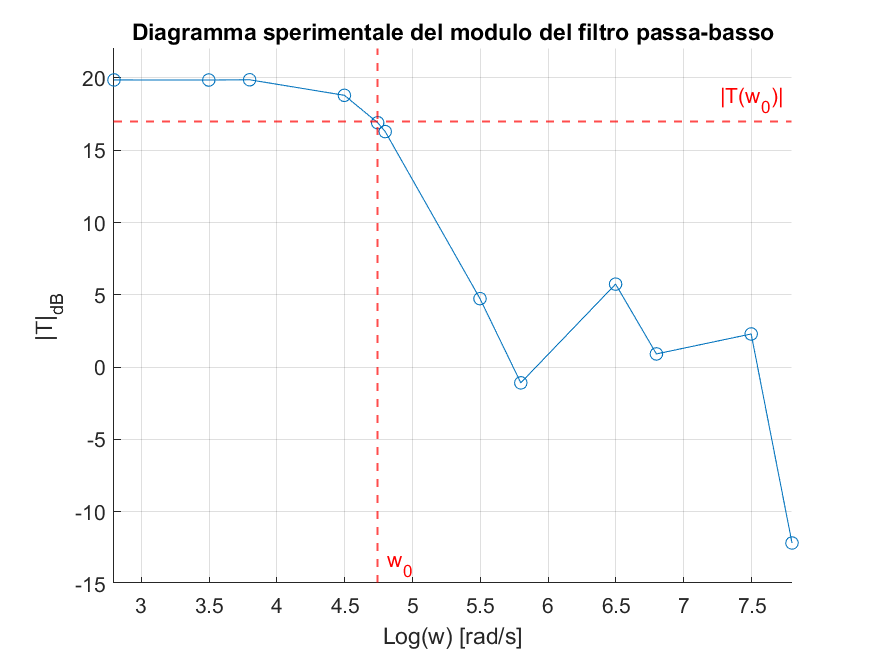
\includegraphics[height=7.3cm]{immagini/modulo_sper}
	\caption{Diagramma di Bode del modulo ottenuto sperimentalmente.}
	\label{figura:modulosperimentale}
\end{figure}
\begin{figure}[h!]
	\centering
	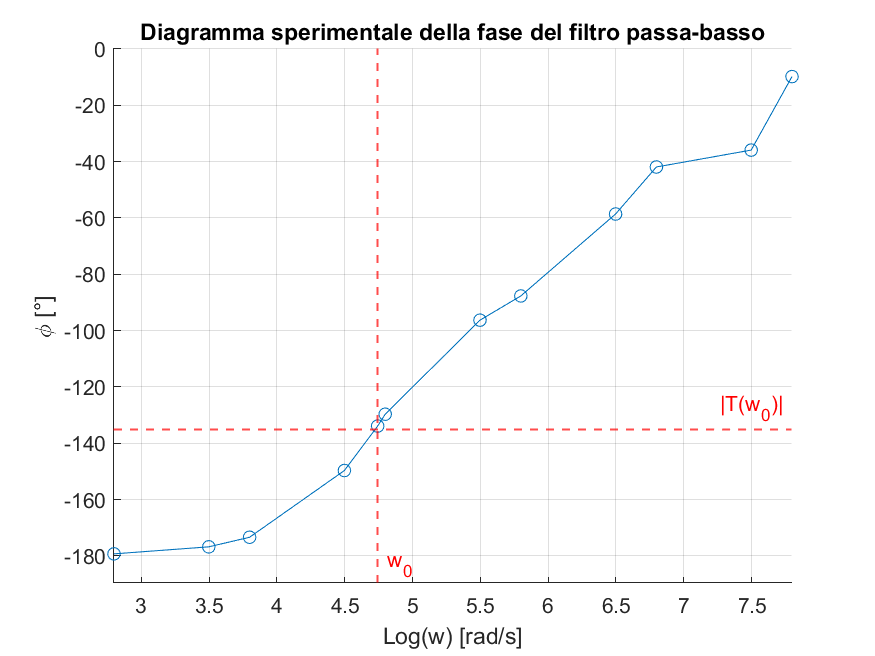
\includegraphics[height=7.3cm]{immagini/fase_sper}
	\caption{Diagramma di Bode della fase ottenuto sperimentalmente.}
	\label{figura:fasesperimentale}
\end{figure}
Come ci aspettavamo, il guadagno in bassa frequenza è pari a \SI{20}{\decibel}, che corrisponde ad un valore di guadagno di 10 in scala lineare. Anche lo sfasamento in bassa frequenza è molto preciso ed è pari a circa \SI{-180}{\degree}. Spostandoci verso la frequenza di taglio, il modulo rimane circa costante e diminuisce di \SI{3}{\decibel} in corrispondenza della frequenza di taglio, esattamente come ci aspettiamo (in scala lineare, \SI{17}{\decibel} corrispondono ad un valore di 7.08, valore molto prossimo al guadagno ricavato, che è 7.00). Oltre questa frequenza, il modulo inizia a diminuire. Per quanto riguarda invece la fase, spostandoci verso la frequenza di taglio il suo valore aumenta, fino a raggiungere il valore \SI{-133}{\degree} in corrispondenza della frequenza di taglio. Questo valore è molto vicino allo sfasamento di \SI{-135}{\degree} che ci aspettiamo dall'analisi teorica. Proseguendo verso frequenze crescenti, la fase continua ad aumentare. \par
\begin{figure}[h!]
	\centering
	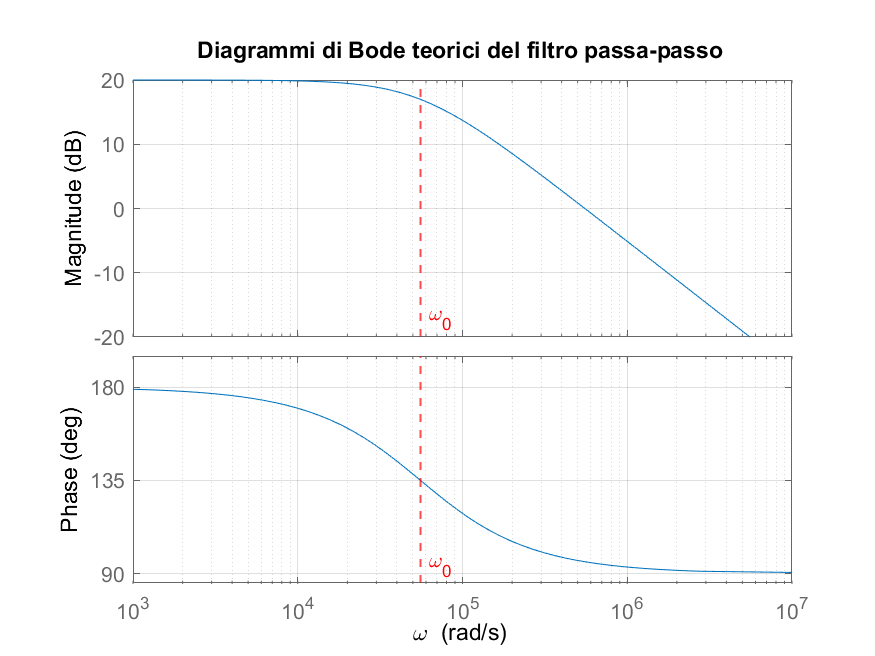
\includegraphics[height=7.7cm]{immagini/Bode_teo}
	\caption{Diagrammi di Bode teorici.}
	\label{figura:bodeteorici}
\end{figure}
Per analizzare le prestazioni del filtro, confrontiamo i diagrammi sperimentali con quelli teorici, mostrati in figura \ref{figura:bodeteorici}. Possiamo notare che sia il diagramma sperimentale del modulo che quello della fase approssimano molto bene i diagrammi teorici solo fino ad una frequenza di \SI{100}{k\hertz}. Oltre questa frequenza, il grafico sperimentale del modulo oscilla tra valori di \SI{5}{\decibel} e \SI{0}{\decibel} per poi calare drasticamente alla frequenza di \SI {10}{M\hertz}. Il comportamento teorico prevede invece che il modulo diminuisca linearmente con una pendenza di \SI{-20}{\decibel}/decade. Oltre la frequenza di \SI{100}{k\hertz} anche il diagramma sperimentale della fase non segue più il comportamento teorico: invece che assestarsi asintoticamente al valore di \SI{90}{\degree} (\SI{-90}{\degree} nel nostro diagramma), la fase aumenta pressoché linearmente. Questo risultato apparentemente anomalo può essere spiegato se consideriamo il comportamento in alta frequenza dell'amplificatore operazionale che utilizziamo per realizzare il filtro: dato che l'OPAMP è un componente reale e non ideale, ha delle limitazioni in frequenza ed il suo comportamento è di tipo passa-basso, motivo per cui dopo una certa frequenza il nostro circuito non è più in grado di funzionare ed amplificare correttamente. In figura \ref{figura:TEK13} vediamo che quando applichiamo una sinusoide con tensione picco-picco di \SI{500}{m\volt} e frequenza \SI{10}{M\hertz} l'uscita non è più in controfase rispetto all'ingresso ed è inoltre fortemente attenuata.
\begin{figure}[h!]
	\centering
	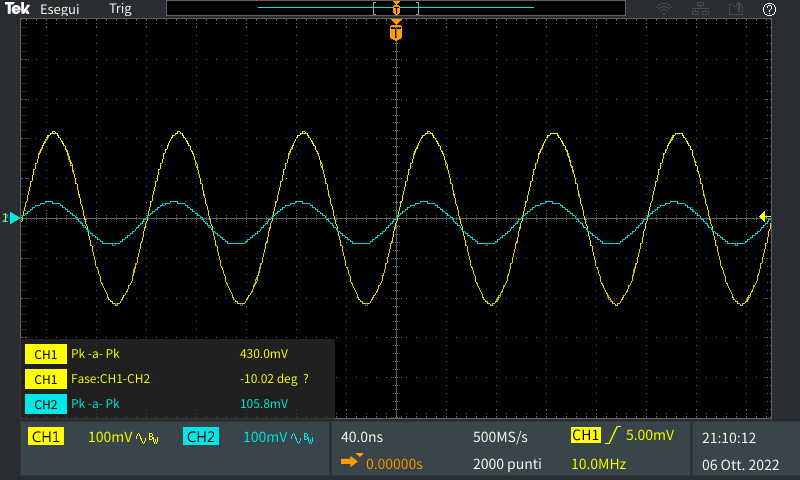
\includegraphics[height=6.5cm]{immagini/TEK00013}
	\caption{Risposta del circuito ad una sinusoide ad alta frequenza.}
	\label{figura:TEK13}
\end{figure}
\\Se guardiamo il datasheet, vediamo che l'amplificatore operazionale \textmu A741 ha prodotto banda-guadagno di \SI{1}{M\hertz}, questo valore corrisponde alla banda passante dell'OPAMP in configurazione ad anello aperto. Nel grafico seguente, la figura \ref{figura:bandaguad}, è riportato il grafico del guadagno in anello aperto del nostro componente. Noi però non lo utilizziamo in anello aperto, bensì in configurazione invertente con un guadagno di \SI{20}{\decibel}, quindi la banda passante dell'amplificatore si riduce, il suo valore si determina andando a vedere a quale frequenza il grafico del guadagno in anello aperto attraversa la linea a \SI{20}{\decibel}. La banda passante è di \SI{100}{k\hertz}, questo è perfettamente in accordo con il comportamento del circuito che osserviamo, perché fino a questa frequenza i diagrammi di Bode sperimentali di modulo e fase sono sovrapponibili ai diagrammi teorici, oltre questa frequenza invece subentrano le non-idealità dell'amplificatore operazionale e di conseguenza il comportamento reale differisce da quello teorico ideale.
\begin{figure}[h!]
	\centering
	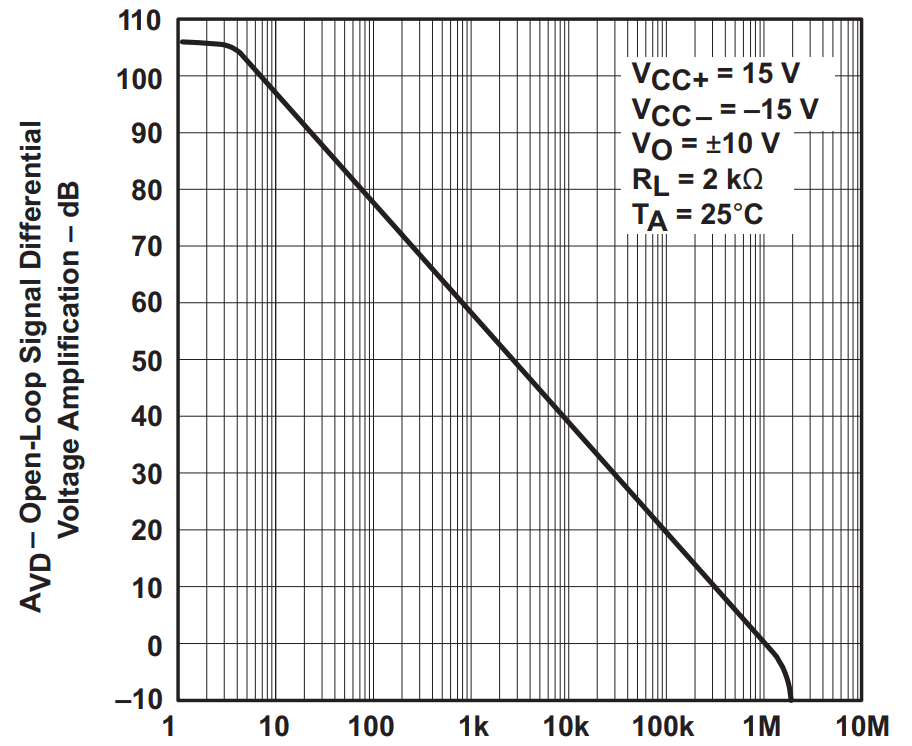
\includegraphics[height=6cm]{immagini/gbw}
	\caption{Grafico del guadagno in anello aperto dell'\textmu A741. Fonte: datasheet.} % metti link
	\label{figura:bandaguad}
\end{figure}
\\La limitazione in frequenza non è l'unica non idealità dell'amplificatore operazionale che possiamo osservare. L'uscita di un OPAMP non può assumere dei valori di tensione (in modulo) grandi a piacere, ma è limitata dalle alimentazioni: se l'uscita dovesse essere maggiore dell'alimentazione positiva, il segnale satura al valore dell'alimentazione positiva, al contrario, se l'uscita dovesse essere più negativa dell'alimentazione negativa, satura al valore di questa alimentazione. Tuttavia, in un amplificatore operazionale reale, la saturazione subentra prima che si raggiungano le alimentazioni, in generale la tensione di saturazione positiva è diversa dalla tensione di saturazione negativa perché lo schema interno dell'OPAMP non è simmetrico. \par % AGG
Dalla figura \ref{figura:satur} si può notare che quando applichiamo in ingresso una sinusoide di frequenza \SI{1}{k\hertz} e tensione picco-picco di \SI{5}{\volt} il segnale in uscita satura. In particolare questo evento si verifica per le semionde negative del segnale in uscita quando la tensione picco-picco del segnale in ingresso ha un valore superiore a \SI{1.7}{\volt}, mentre per le semionde positive del segnale in uscita si verifica quando la tensione picco-picco del segnale in ingresso ha un valore superiore a \SI{2}{\volt}. \par
Sempre da questo grafico, notiamo un'altra non idealità dell'amplificatore operazionale, che è la tensione di offset. Infatti, quando l'ingresso è pari a \SI{0}{\volt} l'uscita non si trova ad un valore di tensione nullo ma positivo, perché in un OPAMP reale l'offset di tensione, seppur piccolo, non è nullo. % MOD vediamo se lasciare o togliere
\begin{figure}[h!]
	\centering
	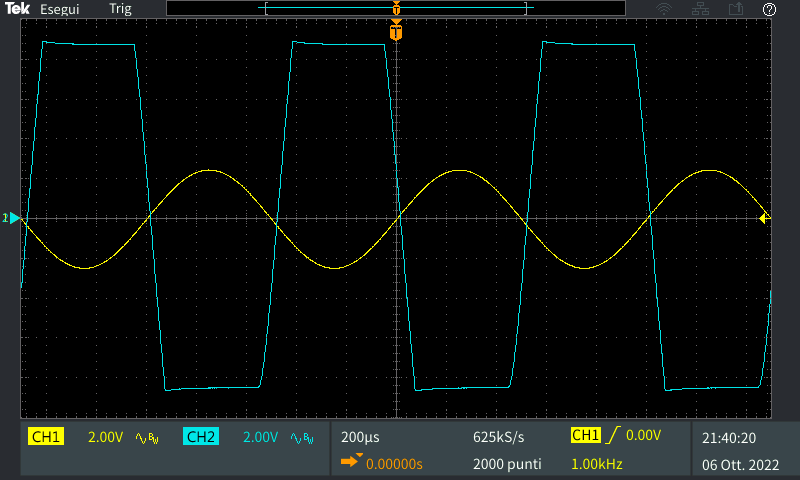
\includegraphics[height=6.5cm]{immagini/TEK00015}
	\caption{Grafico della tensione in uscita quando si verifica la saturazione.}
	\label{figura:satur}
\end{figure}
\\Per ultimo, si è analizzato il comportamento del circuito quando il segnale in ingresso presenta un offset di tensione. Abbiamo quindi applicato in ingresso una sinusoide con tensione picco-picco di \SI{500}{m\volt}, offset DC di \SI{+100}{m\volt} e  frequenza di \SI{1}{k\hertz}. Analizziamo la risposta del circuito, accoppiando l'oscilloscopio prima in DC e poi in AC. Il grafico della tensione in uscita al circuito nei due casi è riportato in figura \ref{figura:accopp}. \par
\begin{figure}
\centering
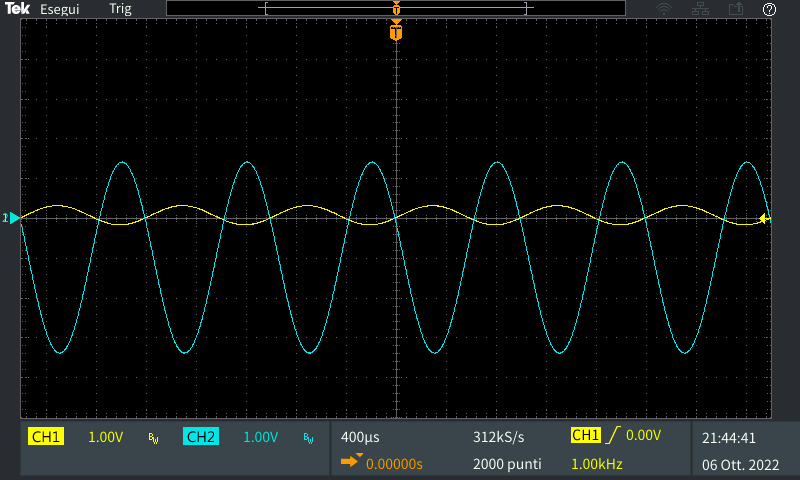
\includegraphics[height=6.5cm]{immagini/TEK00018}\\(a)\\[1ex]
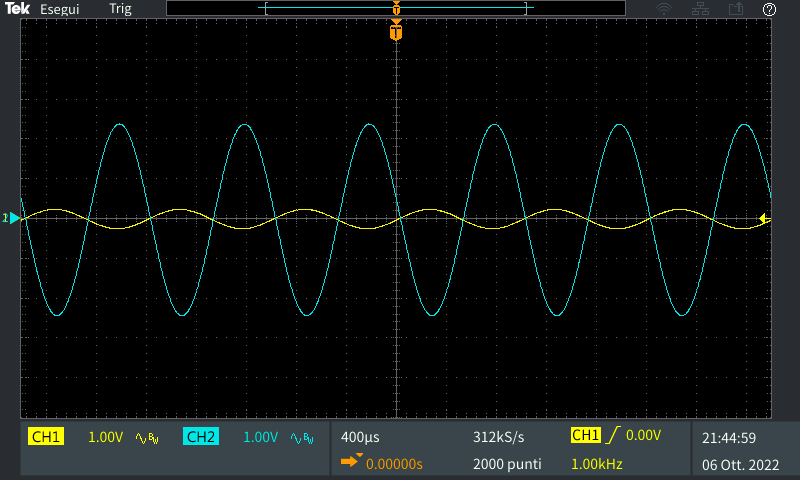
\includegraphics[height=6.5cm]{immagini/TEK00019}\\(b)
\caption{Risposta del circuito con accoppiamento DC (a) e accoppiamento AC (b).}
	\label{figura:accopp}
\end{figure}
% offset = +100 mV
Dal primo grafico, possiamo notare che sia l'ingresso che l'uscita presentano un offset in DC. In particolare, anche l'offset viene amplificato di un fattore pari al guadagno del circuito, perciò la sinusoide in uscita, oltre che essere amplificata, sarà traslata di \SI{-1}{\volt} sull'asse delle ordinate. Per analizzare soltanto la componente di segnale, senza l'offset, possiamo sfruttare l'oscilloscopio: se accoppiamo entrambe le sonde in AC, l'oscilloscopio ``cancella'' l'offset di tensione e in uscita vediamo solo la componente di segnale, come illustrato nel secondo grafico di figura \ref{figura:accopp}.

%----------------------------------------------------------------------------------------

\end{document}
